\documentclass[10pt,a4paper]{amsart}
\usepackage[margin=19mm]{geometry}
\usepackage{amsmath,amssymb,mathtools}
\usepackage[scr=rsfs,cal=euler]{mathalfa}
\usepackage{xfrac}
\usepackage[unicode,hidelinks,bookmarks=false]{hyperref}
\newcommand{\ie}{i.e.\ }
\newcommand{\cf}{cf.\ }
\newcommand{\resp}{respectively\ }
\newcommand{\Subsection}{\subsection}
\providecommand{\nobreakdash}{\nobreak\hbox{-}}
\setlength{\emergencystretch}{2em}
\multlinegap0pt
% ---------------------------------------------------------------------------
% Editorial AMS wrapper prelude. The theorem environments and the mathematical macros below are
% transcribed from the paper's own preamble (cached-originals/source0.tex lines 27--202); the AMS amsart
% class, the named format packages of the pinned TeX Live runtime and this editorial formatting are not
% part of the author's text. No mathematics is changed.
% ---------------------------------------------------------------------------
\usepackage{bbm}
\usepackage{dsfont}
\usepackage{upgreek}
\usepackage{cancel}
\usepackage{tikz-cd}
\newcommand{\nn}{\nonumber}
\newcommand{\dd}{{\rm d}}
\newcommand{\w}{\wedge}
\newtheorem{theorem}{Theorem}[section]
\newtheorem{lemma}[theorem]{Lemma}
\newtheorem{proposition}[theorem]{Proposition}
\newtheorem{definition}[theorem]{Definition}
\newtheorem{corollary}[theorem]{Corollary}





	







\newcommand{\Cbb}{\mathbb{C}}
\newcommand{\Zbb}{\mathbb{Z}}


\newcommand\vPsi {|\Psi\rangle}
\newcommand\vPhi {|\Phi\rangle}

\newcommand{\CG}{\mathbb{C}[G]}
\newcommand{\CGdual}{\mathbb{C}[G]^{\vee}}

\newcommand{\identity}{\mathds{1}}

\newcommand{\ZJ}[1]{{\color{blue!40} Zhian: #1}}%


\newcommand{\cN}{\mathcal{N}}
\newcommand{\Acal}{\mathcal{A}}

\newcommand{\be}{\begin{equation}}
	\newcommand{\ee}{\end{equation}}
\def\bea#1\eea{\begin{align}#1\end{align}}
\newcommand{\tr}{{\rm tr}}
























\renewcommand{\qedsymbol}{$\blacksquare$}

\theoremstyle{definition}
\newtheorem{example}{Example}

\theoremstyle{remark}
\newtheorem{remark}{Remark}[section]

\theoremstyle{remark}
\newtheorem{notation}{Notation}[section]


\newcommand\EB{\EuScript{B}}
\newcommand\EC{\EuScript{C}}
\newcommand\ED{\EuScript{D}}
\newcommand\EE{\EuScript{E}}
\newcommand\EM{\EuScript{M}}
\newcommand\EN{\EuScript{N}}
\newcommand\EP{\EuScript{P}}
\newcommand\ES{\EuScript{S}}
\newcommand\ER{\EuScript{R}}
\newcommand\EW{\EuScript{W}}

\newcommand{\LA}{\mathcal{A}}

\newcommand{\Hilb}{\mathsf{Hilb}}
\newcommand\Fun{\textsf{Fun}}
\newcommand\Vect{\textsf{Vect}}
\newcommand\hilb  {\textsf{Hilb}}
\newcommand\Rep {\mathsf{Rep}}

\newcommand\Obj {\mathrm{Obj}}
\newcommand\id {\mathrm{id}}
\newcommand\Irr {\mathrm{Irr}}
\newcommand\End {\mathrm{End}}
\newcommand\Hom {\mathrm{Hom}}
\newcommand{\one}{\mathbbm{1}}
\newcommand\rmod{\textsf{RMod}}
\newcommand\Mod{\textsf{Mod}}
\newcommand\AModA{_A\textsf{Mod}_A}
\newcommand{\Zp}{\mathbb{Z}_p}
\newcommand{\Ztwo}{\mathbb{Z}_2}
\newcommand{\RMod}{\mathsf{RMod}}
\newcommand{\FPdim}{\operatorname{FPdim}}
\newcommand{\Aut}{\operatorname{Aut}}
\newcommand{\CC}{\mathsf{CC}_{\Zbb_2}}


\newcommand\Hhat {\hat{H}}
\newcommand\hhat {\hat{h}}
\newcommand\Jhat {\hat{J}}














\begin{document}
\title{Topological quantum color code model on infinite lattice}
\author{Shiyu Cao, Zhian Jia and Sheng Tan}
\date{Source: arXiv:2601.12409v3; distributed under CC BY 4.0}
\maketitle
\noindent\emph{Source, version and licence.} \emph{Topological quantum color code model on infinite lattice}, by Shiyu Cao, Zhian Jia and Sheng Tan. The source of this editable unit is the e-print of \textbf{version v3} of arXiv:2601.12409, https://arxiv.org/abs/2601.12409v3, whose material is distributed under the Creative Commons Attribution 4.0 International licence, http://creativecommons.org/licenses/by/4.0/, as recorded in the arXiv licence metadata for this paper and shown on that abstract page. The whole of the body below is version v3, the newest version of the paper. Full rights notice: licenses/arxiv-2601.12409-CC-BY-4.0.txt.\par\smallskip
\noindent\textit{Editorial scope.} Counted unit: original Theorem 3.22 of the article, the statement carried by the source environment \texttt{theorem} with source label \texttt{thm:category\_equivalence}, cached-originals/source0.tex lines 1553--1555, printed as \textbf{Theorem 3.22} exactly as in the article, and described there as the main result of the paper. It is delivered together with the authors' own complete proof as the single primary proof body, source0.tex lines 1558--1609 (52 lines): the \texttt{proof} environment that immediately follows the statement and carries out the comparison of the two braided tensor categories. No proof marker is added and no mathematics is written, repaired or re-derived; the authors' notation and the printed slips of the source are kept literal. Necessary complete context is retained uncounted: source0.tex lines 534--536 and 539--580 are \emph{not} retained, and the closure of the counted statement and proof over references and citations was computed: it contains no reference and no citation at all, so the delivered passages are the statement and its proof together with nothing else, every reference inside them resolving inside the delivered file. The article's own numbering is reproduced by explicit counter settings: the counter \texttt{theorem}, declared by \texttt{\textbackslash newtheorem\{theorem\}\{Theorem\}[section]} with lemma, proposition, definition and corollary sharing it, is set before each retained passage, so the counted statement prints as Theorem 3.22 exactly as in the article. No \texttt{\textbackslash cite} command occurs in any retained passage, so this unit delivers no bibliography entry; the article's own bibliography data file \texttt{mybib.bib} is neither spliced into the bundled source nor redistributed. The retained passages contain no figure environment and no graphics-inclusion command, so no artwork is redistributed, and none of the artwork shipped by the e-print is used. The source's own class is the standard \texttt{article} class; the e-print ships the authors' own style file \texttt{JiaHep.sty}, which is not shipped, loaded or redistributed here (the mathematical macros the retained passages need are transcribed from the paper's own preamble instead), and no publisher class is shipped, used or redistributed. Every declared body of this unit is an exact, unmodified span of source0.tex: no body is a bounded passage comparison, \texttt{omit} was not used anywhere, and consequently no fidelity receipt is asserted in delivery-evidence.json. The complete concatenated original source is bundled as sources/192943/source0.tex. Omitted from this editable unit and therefore absent from it are source0.tex lines 1--697; 727--748; 778--1212; 1217--1286; 1307--1497; 1502--1506; 1513--1552; 1556--1557; 1610--2409, that is the article's own preamble, title and author block and abstract, the introduction, the sections on states and on the local structure of the model, the remaining superselection sector theorems with their proofs, the appendix reviewing the representation category of the quantum double, and the article's bibliography data, all of which remain present in the bundled source but are not delivered here. The AMS \texttt{amsart} wrapper, the named format packages of the pinned TeX Live runtime and this editorial source, licence and scope paragraph are editorial formatting only.\par\smallskip
\setcounter{section}{3}
\setcounter{equation}{0}
\setcounter{example}{0}
\setcounter{notation}{0}
\setcounter{remark}{0}
\setcounter{theorem}{0}
\begin{table}[h!]
\centering
\resizebox{\textwidth}{!}{
\begin{tabular}{c|cccccccccccccccc}
\hline\hline
$\otimes$ & $\mathbbm{1}$ & $\mathtt{rx}$ & $\mathtt{ry}$ & $\mathtt{rz}$ & $\mathtt{gx}$ & $\mathtt{gy}$ & $\mathtt{gz}$ & $\mathtt{bx}$ & $\mathtt{by}$ & $\mathtt{bz}$ & $\mathtt{f}_1$ & $\mathtt{f}_2$ & $\mathtt{f}_3$ & $\mathtt{f}_4$ & $\mathtt{f}_5$ & $\mathtt{f}_6$ \\
\hline
$\mathbbm{1}$ & $\mathbbm{1}$ & $\mathtt{rx}$ & $\mathtt{ry}$ & $\mathtt{rz}$ & $\mathtt{gx}$ & $\mathtt{gy}$ & $\mathtt{gz}$ & $\mathtt{bx}$ & $\mathtt{by}$ & $\mathtt{bz}$ & $\mathtt{f}_1$ & $\mathtt{f}_2$ & $\mathtt{f}_3$ & $\mathtt{f}_4$ & $\mathtt{f}_5$ & $\mathtt{f}_6$ \\
$\mathtt{rx}$ & $\mathtt{rx}$ & $\mathbbm{1}$ & $\mathtt{rz}$ & $\mathtt{ry}$ & $\mathtt{bx}$ & $\mathtt{f}_5$ & $\mathtt{f}_6$ & $\mathtt{gx}$ & $\mathtt{f}_4$ & $\mathtt{f}_1$ & $\mathtt{bz}$ & $\mathtt{f}_3$ & $\mathtt{f}_2$ & $\mathtt{by}$ & $\mathtt{gy}$ & $\mathtt{gz}$ \\
$\mathtt{ry}$ & $\mathtt{ry}$ & $\mathtt{rz}$ & $\mathbbm{1}$ & $\mathtt{rx}$ & $\mathtt{f}_2$ & $\mathtt{by}$ & $\mathtt{f}_1$ & $\mathtt{f}_3$ & $\mathtt{gy}$ & $\mathtt{f}_6$ & $\mathtt{gz}$ & $\mathtt{gx}$ & $\mathtt{bx}$ & $\mathtt{f}_5$ & $\mathtt{f}_4$ & $\mathtt{bz}$ \\
$\mathtt{rz}$ & $\mathtt{rz}$ & $\mathtt{ry}$ & $\mathtt{rx}$ & $\mathbbm{1}$ & $\mathtt{f}_3$ & $\mathtt{f}_4$ & $\mathtt{bz}$ & $\mathtt{f}_2$ & $\mathtt{f}_5$ & $\mathtt{gz}$ & $\mathtt{f}_6$ & $\mathtt{bx}$ & $\mathtt{gx}$ & $\mathtt{gy}$ & $\mathtt{by}$ & $\mathtt{f}_1$ \\
$\mathtt{gx}$ & $\mathtt{gx}$ & $\mathtt{bx}$ & $\mathtt{f}_2$ & $\mathtt{f}_3$ & $\mathbbm{1}$ & $\mathtt{gz}$ & $\mathtt{gy}$ & $\mathtt{rx}$ & $\mathtt{f}_1$ & $\mathtt{f}_4$ & $\mathtt{by}$ & $\mathtt{ry}$ & $\mathtt{rz}$ & $\mathtt{bz}$ & $\mathtt{f}_6$ & $\mathtt{f}_5$ \\
$\mathtt{gy}$ & $\mathtt{gy}$ & $\mathtt{f}_5$ & $\mathtt{by}$ & $\mathtt{f}_4$ & $\mathtt{gz}$ & $\mathbbm{1}$ & $\mathtt{gx}$ & $\mathtt{f}_6$ & $\mathtt{ry}$ & $\mathtt{f}_3$ & $\mathtt{f}_2$ & $\mathtt{f}_1$ & $\mathtt{bz}$ & $\mathtt{rz}$ & $\mathtt{rx}$ & $\mathtt{bx}$ \\
$\mathtt{gz}$ & $\mathtt{gz}$ & $\mathtt{f}_6$ & $\mathtt{f}_1$ & $\mathtt{bz}$ & $\mathtt{gy}$ & $\mathtt{gx}$ & $\mathbbm{1}$ & $\mathtt{f}_5$ & $\mathtt{f}_2$ & $\mathtt{rz}$ & $\mathtt{ry}$ & $\mathtt{by}$ & $\mathtt{f}_4$ & $\mathtt{f}_3$ & $\mathtt{bx}$ & $\mathtt{rx}$ \\
$\mathtt{bx}$ & $\mathtt{bx}$ & $\mathtt{gx}$ & $\mathtt{f}_3$ & $\mathtt{f}_2$ & $\mathtt{rx}$ & $\mathtt{f}_6$ & $\mathtt{f}_5$ & $\mathbbm{1}$ & $\mathtt{bz}$ & $\mathtt{by}$ & $\mathtt{f}_4$ & $\mathtt{rz}$ & $\mathtt{ry}$ & $\mathtt{f}_1$ & $\mathtt{gz}$ & $\mathtt{gy}$ \\
$\mathtt{by}$ & $\mathtt{by}$ & $\mathtt{f}_4$ & $\mathtt{gy}$ & $\mathtt{f}_5$ & $\mathtt{f}_1$ & $\mathtt{ry}$ & $\mathtt{f}_2$ & $\mathtt{bz}$ & $\mathbbm{1}$ & $\mathtt{bx}$ & $\mathtt{gx}$ & $\mathtt{gz}$ & $\mathtt{f}_6$ & $\mathtt{rx}$ & $\mathtt{rz}$ & $\mathtt{f}_3$ \\
$\mathtt{bz}$ & $\mathtt{bz}$ & $\mathtt{f}_1$ & $\mathtt{f}_6$ & $\mathtt{gz}$ & $\mathtt{f}_4$ & $\mathtt{f}_3$ & $\mathtt{rz}$ & $\mathtt{by}$ & $\mathtt{bx}$ & $\mathbbm{1}$ & $\mathtt{rx}$ & $\mathtt{f}_5$ & $\mathtt{gy}$ & $\mathtt{gx}$ & $\mathtt{f}_2$ & $\mathtt{ry}$ \\
$\mathtt{f}_1$ & $\mathtt{f}_1$ & $\mathtt{bz}$ & $\mathtt{gz}$ & $\mathtt{f}_6$ & $\mathtt{by}$ & $\mathtt{f}_2$ & $\mathtt{ry}$ & $\mathtt{f}_4$ & $\mathtt{gx}$ & $\mathtt{rx}$ & $\mathbbm{1}$ & $\mathtt{gy}$ & $\mathtt{f}_5$ & $\mathtt{bx}$ & $\mathtt{f}_3$ & $\mathtt{rz}$ \\
$\mathtt{f}_2$ & $\mathtt{f}_2$ & $\mathtt{f}_3$ & $\mathtt{gx}$ & $\mathtt{bx}$ & $\mathtt{ry}$ & $\mathtt{f}_1$ & $\mathtt{by}$ & $\mathtt{rz}$ & $\mathtt{gz}$ & $\mathtt{f}_5$ & $\mathtt{gy}$ & $\mathbbm{1}$ & $\mathtt{rx}$ & $\mathtt{f}_6$ & $\mathtt{bz}$ & $\mathtt{f}_4$ \\
$\mathtt{f}_3$ & $\mathtt{f}_3$ & $\mathtt{f}_2$ & $\mathtt{bx}$ & $\mathtt{gx}$ & $\mathtt{rz}$ & $\mathtt{bz}$ & $\mathtt{f}_4$ & $\mathtt{ry}$ & $\mathtt{f}_6$ & $\mathtt{gy}$ & $\mathtt{f}_5$ & $\mathtt{rx}$ & $\mathbbm{1}$ & $\mathtt{gz}$ & $\mathtt{f}_1$ & $\mathtt{by}$ \\
$\mathtt{f}_4$ & $\mathtt{f}_4$ & $\mathtt{by}$ & $\mathtt{f}_5$ & $\mathtt{gy}$ & $\mathtt{bz}$ & $\mathtt{rz}$ & $\mathtt{f}_3$ & $\mathtt{f}_1$ & $\mathtt{rx}$ & $\mathtt{gx}$ & $\mathtt{bx}$ & $\mathtt{f}_6$ & $\mathtt{gz}$ & $\mathbbm{1}$ & $\mathtt{ry}$ & $\mathtt{f}_2$ \\
$\mathtt{f}_5$ & $\mathtt{f}_5$ & $\mathtt{gy}$ & $\mathtt{f}_4$ & $\mathtt{by}$ & $\mathtt{f}_6$ & $\mathtt{rx}$ & $\mathtt{bx}$ & $\mathtt{gz}$ & $\mathtt{rz}$ & $\mathtt{f}_2$ & $\mathtt{f}_3$ & $\mathtt{bz}$ & $\mathtt{f}_1$ & $\mathtt{ry}$ & $\mathbbm{1}$ & $\mathtt{gx}$ \\
$\mathtt{f}_6$ & $\mathtt{f}_6$ & $\mathtt{gz}$ & $\mathtt{bz}$ & $\mathtt{f}_1$ & $\mathtt{f}_5$ & $\mathtt{bx}$ & $\mathtt{rx}$ & $\mathtt{gy}$ & $\mathtt{f}_3$ & $\mathtt{ry}$ & $\mathtt{rz}$ & $\mathtt{f}_4$ & $\mathtt{by}$ & $\mathtt{f}_2$ & $\mathtt{gx}$ & $\mathbbm{1}$ \\
\hline\hline
\end{tabular}
}
\caption{Fusion rules of the 16 anyons of the color code ($\mathsf{CC}_{\mathbb{Z}_2}$), where ``row label'' $\otimes$ ``column label''.}
\label{tab:colorcode_fusion}
\end{table}

\setcounter{section}{3}
\setcounter{equation}{0}
\setcounter{example}{0}
\setcounter{notation}{0}
\setcounter{remark}{0}
\setcounter{theorem}{0}
\begin{table}[t]
\centering
\resizebox{\textwidth}{!}{
\begin{tabular}{c|cccccccccccccccc}
\hline\hline
$M_{a,b}$ & $\mathbbm{1}$ & $\mathtt{rx}$ & $\mathtt{ry}$ & $\mathtt{rz}$ & $\mathtt{gx}$ & $\mathtt{gy}$ & $\mathtt{gz}$ & $\mathtt{bx}$ & $\mathtt{by}$ & $\mathtt{bz}$ & $\mathtt{f}_1$ & $\mathtt{f}_2$ & $\mathtt{f}_3$ & $\mathtt{f}_4$ & $\mathtt{f}_5$ & $\mathtt{f}_6$ \\
\hline
$\mathbbm{1}$ & $+1$ & $+1$ & $+1$ & $+1$ & $+1$ & $+1$ & $+1$ & $+1$ & $+1$ & $+1$ & $+1$ & $+1$ & $+1$ & $+1$ & $+1$ & $+1$ \\
$\mathtt{rx}$ & $+1$ & $+1$ & $+1$ & $+1$ & $+1$ & $-1$ & $-1$ & $+1$ & $-1$ & $-1$ & $-1$ & $+1$ & $+1$ & $-1$ & $-1$ & $-1$ \\
$\mathtt{ry}$ & $+1$ & $+1$ & $+1$ & $+1$ & $-1$ & $+1$ & $-1$ & $-1$ & $+1$ & $-1$ & $-1$ & $-1$ & $-1$ & $+1$ & $+1$ & $-1$ \\
$\mathtt{rz}$ & $+1$ & $+1$ & $+1$ & $+1$ & $-1$ & $-1$ & $+1$ & $-1$ & $-1$ & $+1$ & $+1$ & $-1$ & $-1$ & $-1$ & $-1$ & $+1$ \\
$\mathtt{gx}$ & $+1$ & $+1$ & $-1$ & $-1$ & $+1$ & $+1$ & $+1$ & $+1$ & $-1$ & $-1$ & $-1$ & $-1$ & $-1$ & $-1$ & $+1$ & $+1$ \\
$\mathtt{gy}$ & $+1$ & $-1$ & $+1$ & $-1$ & $+1$ & $+1$ & $+1$ & $-1$ & $+1$ & $-1$ & $+1$ & $+1$ & $-1$ & $-1$ & $-1$ & $-1$ \\
$\mathtt{gz}$ & $+1$ & $-1$ & $-1$ & $+1$ & $+1$ & $+1$ & $+1$ & $-1$ & $-1$ & $+1$ & $-1$ & $-1$ & $+1$ & $+1$ & $-1$ & $-1$ \\
$\mathtt{bx}$ & $+1$ & $+1$ & $-1$ & $-1$ & $+1$ & $-1$ & $-1$ & $+1$ & $+1$ & $+1$ & $+1$ & $-1$ & $-1$ & $+1$ & $-1$ & $-1$ \\
$\mathtt{by}$ & $+1$ & $-1$ & $+1$ & $-1$ & $-1$ & $+1$ & $-1$ & $+1$ & $+1$ & $+1$ & $-1$ & $-1$ & $+1$ & $-1$ & $-1$ & $+1$ \\
$\mathtt{bz}$ & $+1$ & $-1$ & $-1$ & $+1$ & $-1$ & $-1$ & $+1$ & $+1$ & $+1$ & $+1$ & $-1$ & $+1$ & $-1$ & $-1$ & $+1$ & $-1$ \\
$\mathtt{f}_1$ & $+1$ & $-1$ & $-1$ & $+1$ & $-1$ & $+1$ & $-1$ & $+1$ & $-1$ & $-1$ & $+1$ & $+1$ & $-1$ & $+1$ & $-1$ & $+1$ \\
$\mathtt{f}_2$ & $+1$ & $+1$ & $-1$ & $-1$ & $-1$ & $+1$ & $-1$ & $-1$ & $-1$ & $+1$ & $+1$ & $+1$ & $+1$ & $-1$ & $+1$ & $-1$ \\
$\mathtt{f}_3$ & $+1$ & $+1$ & $-1$ & $-1$ & $-1$ & $-1$ & $+1$ & $-1$ & $+1$ & $-1$ & $-1$ & $+1$ & $+1$ & $+1$ & $-1$ & $+1$ \\
$\mathtt{f}_4$ & $+1$ & $-1$ & $+1$ & $-1$ & $-1$ & $-1$ & $+1$ & $+1$ & $-1$ & $-1$ & $+1$ & $-1$ & $+1$ & $+1$ & $+1$ & $-1$ \\
$\mathtt{f}_5$ & $+1$ & $-1$ & $+1$ & $-1$ & $+1$ & $-1$ & $-1$ & $-1$ & $-1$ & $+1$ & $-1$ & $+1$ & $-1$ & $+1$ & $+1$ & $+1$ \\
$\mathtt{f}_6$ & $+1$ & $-1$ & $-1$ & $+1$ & $+1$ & $-1$ & $-1$ & $-1$ & $+1$ & $-1$ & $+1$ & $-1$ & $+1$ & $-1$ & $+1$ & $+1$ \\
\hline\hline
\end{tabular}
}
\caption{Monodromy $M_{a,b}$ for the 16 anyons of the color code.}
\label{tab:colorcode_monodromy}
\end{table}

\setcounter{section}{3}
\setcounter{equation}{2}
\setcounter{example}{0}
\setcounter{notation}{0}
\setcounter{remark}{2}
\setcounter{theorem}{12}
\begin{align}
    \varepsilon_{\rho,\rho'\otimes \rho''}  = (I_{\rho'}\otimes \varepsilon_{\rho,\rho''})(\varepsilon_{\rho,\rho'}\otimes I_{\rho''}), \quad 
    \varepsilon_{\rho\otimes \rho',\rho''}  = (\varepsilon_{\rho,\rho''}\otimes I_{\rho'})(I_\rho\otimes\varepsilon_{\rho',\rho''}). \label{eq:braid_hexagon}
\end{align}

\setcounter{section}{3}
\setcounter{equation}{3}
\setcounter{example}{0}
\setcounter{notation}{0}
\setcounter{remark}{3}
\setcounter{theorem}{14}
\begin{remark}\label{rem:gauge_braiding}
The braiding constructed here is slightly different from that presented in the appendix. 
The two constructions are related by a gauge transformation acting on the fusion/splitting space. 
Since all anyons in the color code are Abelian, these local gauge transformations reduce to complex phase factors. 
Both choices guarantee that the physical observable (the monodromy) is invariant, namely
$\varepsilon_{b,a}\varepsilon_{a,b} = M_{a,b} = R_{b,a} R_{a,b}$. 
In fact, if we choose the three colored strings in the relative positions shown below
\begin{equation*}
    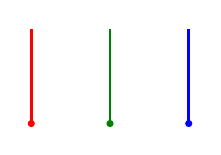
\begin{tikzpicture}
        \draw[red, line width=1pt] (0,0) -- (0,1.2);  
        \path[fill = red] (0,0) circle (1.3pt);
        \draw[green!50!black, line width=1pt] (1,0) -- (1,1.2);  
        \path[fill = green!50!black] (1,0) circle (1.3pt);
        \draw[blue, line width=1pt] (2,0) -- (2,1.2);  
        \path[fill = blue] (2,0) circle (1.3pt);
    \end{tikzpicture}
\end{equation*}
then the braiding $\varepsilon_{a,b}$ defined in this section will satisfy the monodromy in Table~\ref{tab:colorcode_monodromy}. 
One can also show that the braiding $R_{a,b}$ given in the appendix also satisfies this table. 
\end{remark}

\setcounter{section}{3}
\setcounter{equation}{7}
\setcounter{example}{0}
\setcounter{notation}{0}
\setcounter{remark}{5}
\setcounter{theorem}{18}
\begin{theorem}\label{thm:complete_sectors}
    Every irreducible representation satisfying the superselection
    criterion is unitarily equivalent to exactly one of $\pi_0$, $\pi^{ck}$, $\pi^{\mathtt f_i}$ where $c\in\{\mathtt r,\mathtt g,\mathtt b\}$, $k\in\{\mathtt x,\mathtt y,\mathtt z\}$, and $1\leq i\leq6$. 
\end{theorem}

\setcounter{section}{3}
\setcounter{equation}{7}
\setcounter{example}{0}
\setcounter{notation}{0}
\setcounter{remark}{5}
\setcounter{theorem}{19}
\begin{corollary}\label{coro:irreducible_objects_complete}
    Up to unitary equivalence, the irreducible objects of
    $\mathcal D_{\rm loc,tr}$ are precisely $\iota$, $\rho^{ck}$, $\rho^{\mathtt f_i}$, where $\iota$ is the identity endomorphism of $\mathcal A^{au}$, $\rho^{ck}$ denotes a representative of the sector $\pi^{ck}$ localized in the fixed cone $\Lambda_0$, with $c\in\{\mathtt r,\mathtt g,\mathtt b\}$, $k\in\{\mathtt x,\mathtt y,\mathtt z\}$, and $\rho^{\mathtt f_i}$ denotes a representative of the sector
    $\pi^{\mathtt f_i}$ localized in $\Lambda_0$, with
    $1\leq i\leq 6$.
\end{corollary}

\setcounter{section}{3}
\setcounter{equation}{7}
\setcounter{example}{0}
\setcounter{notation}{0}
\setcounter{remark}{5}
\setcounter{theorem}{21}
\begin{theorem}\label{thm:category_equivalence}
    The category $\mathcal D_{\rm loc,tr}^{\rm dual}$ is braided tensor equivalent to the representation category $\Rep(D(\mathbb{Z}_2\times \mathbb{Z}_2))$.
\end{theorem}

\setcounter{section}{3}
\setcounter{equation}{7}
\setcounter{example}{0}
\setcounter{notation}{0}
\setcounter{remark}{5}
\setcounter{theorem}{22}
\begin{proof}
    Denote $G := \mathbb{Z}_2\times \mathbb{Z}_2$. In the appendix, we have included a review of the representation category of the quantum double $D(G)$. Irreducible representations of $D(G)$ are labeled by pairs $(g,\chi)$, $g\in G, \chi\in\widehat{G}$, where $\widehat{G}$ denotes the character group of $G$. 
    Write $G = \{0,a,b,c\}$ where $a+b=c$. Similarly, write $\widehat{G} = \{1,\alpha,\beta,\gamma\}$ where $\alpha\beta=\gamma$. 
    Using these labels, we obtain a full list of $\Irr(\Rep(D(G)))$. Let us denote 
    \begin{align*}
    	& \Pi_\one = (0,1),\; \Pi_{\mathtt{rx}} = (0,\alpha),\; \Pi_{\mathtt{bx}} = (0,\beta),\; \Pi_{\mathtt{gx}} = (0,\gamma), \\
    	& \Pi_{\mathtt{bz}} = (a,1),\; \Pi_{\mathtt{f}_1} = (a,\alpha),\; \Pi_{\mathtt{by}} = (a,\beta),\; \Pi_{\mathtt{f}_4} = (a,\gamma), \\
    	& \Pi_{\mathtt{rz}} = (b,1),\; \Pi_{\mathtt{ry}} = (b,\alpha),\; \Pi_{\mathtt{f}_2} = (b,\beta),\; \Pi_{\mathtt{f}_3} = (b,\gamma), \\
    	& \Pi_{\mathtt{gz}} = (c,1),\; \Pi_{\mathtt{f}_6} = (c,\alpha),\; \Pi_{\mathtt{f}_5} = (c,\beta),\; \Pi_{\mathtt{gy}} = (c,\gamma). 
    \end{align*}
    With these new labels, one can verify that their fusion rules are exactly as shown in Table~\ref{tab:colorcode_fusion}. 
    For example, $\Pi_{\mathtt{rx}}\otimes\Pi_{\mathtt{ry}} = (0,\alpha)\otimes(b,\alpha) = (b,1) = \Pi_{\mathtt{rz}}$, $\Pi_{\mathtt{f}_1}\otimes \Pi_{\mathtt{f}_2} = (a,\alpha)\otimes (b,\beta)  = (c,\gamma) = \Pi_{\mathtt{gy}}$, $\Pi_{\mathtt{ry}}\otimes \Pi_{\mathtt{bz}} = (b,\alpha)\otimes (a,1) = (c,\alpha) = \Pi_{\mathtt{f}_6}$, etc. 
    Let $R_{i,j}$ denote the braiding $\Pi_i\otimes \Pi_j\to \Pi_j\otimes \Pi_i$. Up to a gauge transformation on the fusion/splitting spaces (cf.~Remark~\ref{rem:gauge_braiding}), one has the following nontrivial braiding among the nine bosons $R_{\mathtt{bz},\mathtt{rx}}$, $R_{\mathtt{by},\mathtt{rx}}$, $R_{\mathtt{gz},\mathtt{rx}}$, $ R_{\mathtt{gy},\mathtt{rx}}$, $R_{\mathtt{ry},\mathtt{bx}}$, $R_{\mathtt{bz},\mathtt{ry}}$, $R_{\mathtt{ry},\mathtt{gx}}$, $R_{\mathtt{gz},\mathtt{ry}}$, $R_{\mathtt{rz},\mathtt{bx}}$, $R_{\mathtt{rz},\mathtt{by}}$, $R_{\mathtt{rz},\mathtt{gx}}$, $R_{\mathtt{rz},\mathtt{gy}}$, all of which equal $-1$. 
    The braiding for which at least one of the indices equals $\mathtt{f}_i$ can be calculated using the braiding identities \eqref{eq:braid_hexagon}.

    On the side of $\mathcal{D}_{\rm loc, tr}^{\rm dual}$, choose three half-infinite colored strings with relative positions as shown in Remark~\ref{rem:gauge_braiding}. 
    In this case,  the braiding $\varepsilon_{\mathtt{bz},\mathtt{rx}}$, $\varepsilon_{\mathtt{by},\mathtt{rx}}$, $\varepsilon_{\mathtt{gz},\mathtt{rx}}$, $\varepsilon_{\mathtt{gy},\mathtt{rx}}$, $\varepsilon_{\mathtt{ry},\mathtt{bx}}$, $\varepsilon_{\mathtt{bz},\mathtt{ry}}$, $\varepsilon_{\mathtt{ry},\mathtt{gx}}$, $\varepsilon_{\mathtt{gz},\mathtt{ry}}$, $\varepsilon_{\mathtt{rz},\mathtt{bx}}$, $\varepsilon_{\mathtt{rz},\mathtt{by}}$, $\varepsilon_{\mathtt{rz},\mathtt{gx}}$, 
    $\varepsilon_{\mathtt{rz},\mathtt{gy}}$ for corresponding endomorphisms are all equal to $-\mathds{1}$. 
    Here, for example, $\varepsilon_{\mathtt{bz},\mathtt{rx}}$ denotes the intertwiner $\rho^{\mathtt{bz}}\otimes \rho^{\mathtt{rx}} \to \rho^{\mathtt{rx}}\otimes \rho^{\mathtt{bz}}$.
    Let us define a functor 
    \[
        \Phi:\Rep(D(G)) \to \mathcal{D}_{\rm loc, tr}^{\rm dual}. 
    \]
    On the level of irreducible objects, define $\Phi(\Pi_k) = \rho^k$, where $k$ runs over all 16 labels, and $\rho^k$ corresponds to half-strings of type $k$. 
    Since each $\Pi_k$ is of dimension $1$, $\Hom(\Pi_k,\Pi_j) = \delta_{k,j}\mathbb{C}$. 
    % Fix a nonzero $\lambda_k\in \End(\Pi_k)$ for each $k$. 
    Then on the level of morphisms, define $\Phi(\lambda) = \lambda\mathds{1}_k$ for $\lambda\in \Hom(\Pi_k,\Pi_k)$. 
    Since $\Rep(D(G))$ is semisimple, every object is a finite direct sum of the sixteen irreducible representations above. We therefore extend $\Phi$ additively. 
    For a representation $X = \oplus_k m_k\Pi_k$, define $\Phi(X) = \oplus_k m_k\rho^k$. Here all multiplicities $m_k$ are finite. For two representations $X=\oplus_k m_k\Pi_k$ and $Y= \oplus_k n_k\Pi_k$, we have $\Hom(X,Y) \cong \oplus_k M_{n_k\times m_k}(\mathbb C)$. 
    For $T=(T_k)_k\in\Hom(X,Y)$, 
    define $\Phi(T)=\oplus_k\bigl(T_k\otimes\mathds{1}_{\rho^k}\bigr)$.  
    This defines a functor of Abelian categories. 
    For representations $X,Y\in \Rep(D(G))$, define $J_{X,Y}:\Phi(X\otimes Y) \to \Phi(X)\otimes \Phi(Y)$ by $J_{X,Y}=\mathds{1}$; and define $\varphi:\iota \to \Phi(\Pi_{\one})$ by $\varphi = \mathds{1}$. 
    These data make $\Phi$ a monoidal functor, and it is direct to check that $\Phi$ preserves the relevant tensor category structures. 
    Moreover, it is straightforward but tedious to verify that $\Phi$ preserves the braiding; for example, the diagram
    \begin{equation*}
        \begin{tikzcd}
        	{\Phi(\Pi_{\mathtt{ry}}\otimes\Pi_{\mathtt{bx}})} & {\Phi(\Pi_{\mathtt{bx}}\otimes\Pi_{\mathtt{ry}})} \\
        	{\Phi(\Pi_{\mathtt{ry}})\otimes \Phi(\Pi_{\mathtt{bx}})} & {\Phi(\Pi_{\mathtt{bx}})\otimes\Phi(\Pi_{\mathtt{ry}})}
        	\arrow["{\Phi(R_{\mathtt{ry},\mathtt{bx}})}", from=1-1, to=1-2]
        	\arrow["{J_{\mathtt{ry},\mathtt{bx}}}"', from=1-1, to=2-1]
        	\arrow["{J_{\mathtt{bx},\mathtt{ry}}}", from=1-2, to=2-2]
        	\arrow["{\varepsilon_{\mathtt{ry},\mathtt{bx}}}", from=2-1, to=2-2]
        \end{tikzcd}
    \end{equation*}
    commutes, since $J_{\mathtt{ry},\mathtt{bx}} = J_{\mathtt{bx},\mathtt{ry}} = \mathds{1}$, $\varepsilon_{\mathtt{ry},\mathtt{bx}} = -\mathds{1}$, and $\Phi(R_{\mathtt{ry},\mathtt{bx}}) = R_{\mathtt{ry},\mathtt{bx}}\mathds{1} = -\mathds{1}$. 
    Thus $\Phi$ is a braided tensor functor $\Phi:\Rep(D(G)) \to \mathcal D_{\rm loc,tr}^{\rm dual}$. It is fully faithful, since the sixteen objects $\rho^k$ are pairwise inequivalent irreducible objects and $\Hom(\rho^k,\rho^\ell) = \delta_{k,\ell}\mathbb C$. It remains to verify essential surjectivity. By Theorem~\ref{thm:complete_sectors} (or equivalently Corollary~\ref{coro:irreducible_objects_complete}), the sixteen objects $\rho^k$ form the complete list of irreducible objects of $\mathcal D_{\rm loc,tr}^{\rm dual}$. As observed above, every object of $\mathcal D_{\rm loc,tr}^{\rm dual}$ is a finite direct sum of these irreducible objects. Hence every object of $\mathcal D_{\rm loc,tr}^{\rm dual}$ is isomorphic to an object in the image of $\Phi$. Therefore $\Phi$ is a braided tensor equivalence
    \[
        \Rep(D(G)) \simeq_{\rm br,\otimes} \mathcal D_{\rm loc,tr}^{\rm dual}.
    \]
    This completes the proof. 
\end{proof}

\end{document}
